\chapter{Introdução}
\label{chap:intro}

A crescente adoção de tecnologias como Internet das Coisas (IoT), sistemas de monitoramento industrial e aplicações financeiras em tempo real tem gerado um volume sem precedentes de dados temporais, criando desafios críticos para infraestruturas de armazenamento e análise.

\begin{figure}[h]
    \centering
    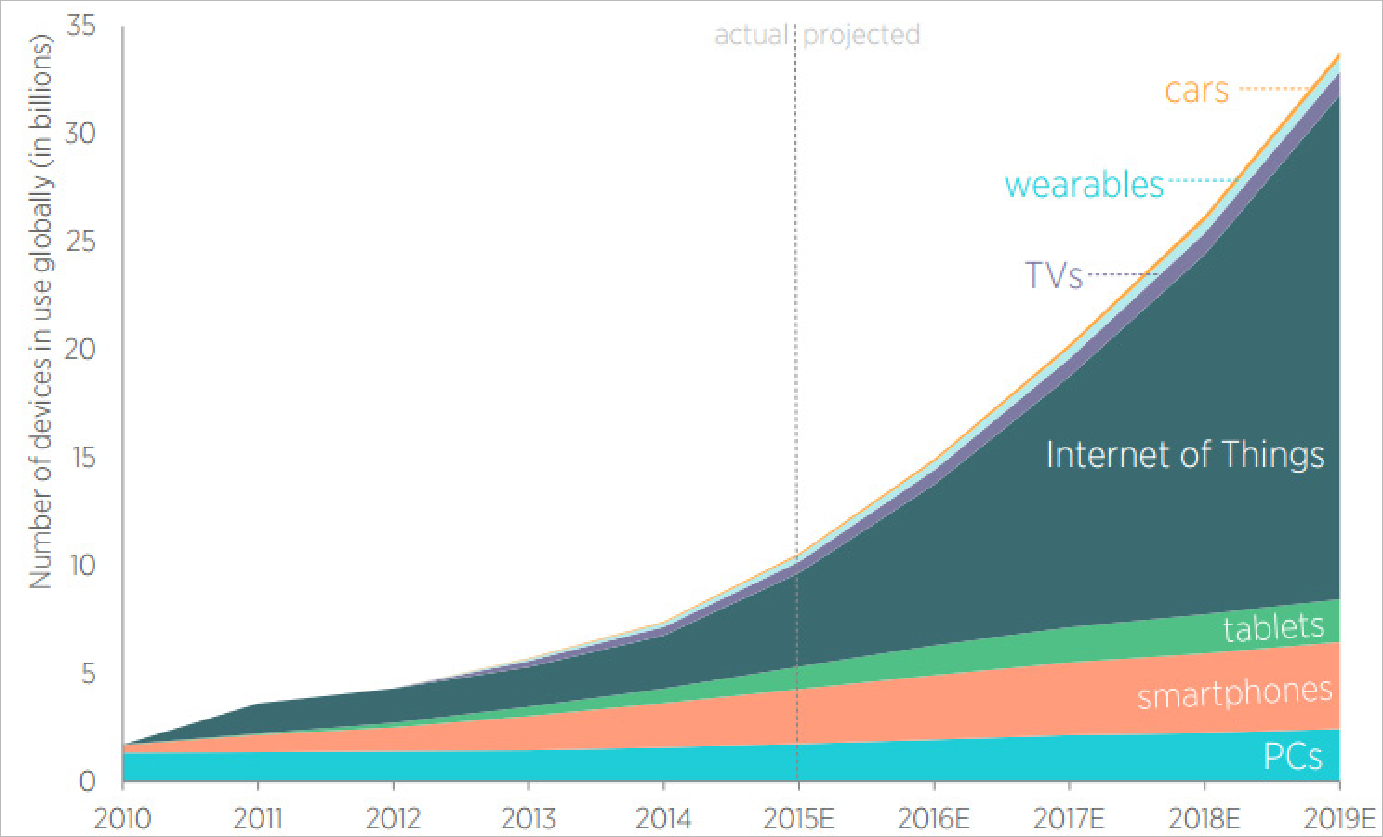
\includegraphics[width=1\textwidth]{figuras/projecao-iot.png}
    \caption{IoT: Dispositivos em uso globalmente}
    \label{fig:projecao_iot}
\end{figure}

A Figura \ref{fig:projecao_iot}, de \citeonline{thierer2015iot}, demonstra que, com a revolução digital, uma explosão na geração de dados temporais vem transformando profundamente a maneira como organizações coletam, armazenam e analisam informações. O gráfico também sugere que o número de dispositivos IoT conectados deve aumentar ainda mais nos próximos anos.

Segundo \citeonline{palma2016}, diversos setores passaram a depender da capacidade de processar fluxos contínuos de dados. Entre eles, destacam-se: o setor financeiro, que utiliza essa tecnologia para analisar flutuações de ações e volumes de transações; o de serviços de transporte, que a emprega no monitoramento de viagens e migrações sazonais; o da medicina, para acompanhar a disseminação de doenças e vírus; e o da análise meteorológica, que permite o uso de dados históricos para previsões mais precisas.

Esses fluxos são sequências de eventos ou medições que são naturalmente ordenadas e indexadas pelo tempo, com precisão de milissegundos. Essa avalanche de informações sequenciais expôs as limitações fundamentais dos bancos de dados tradicionais quando confrontados com padrões de acesso temporal, ingestão em alta velocidade e armazenamento eficiente de históricos de longo prazo.

Neste cenário desafiador, os bancos de dados de séries temporais (TSDBs) emergiram como soluções especializadas, arquitetadas desde sua concepção para atender às exigências únicas dos dados temporais. Ao contrário dos sistemas de propósito geral, os TSDBs incorporam em seu núcleo mecanismos otimizados para compressão temporal, indexação baseada em intervalos e processamento eficiente de operações temporais.

Bancos de dados de séries temporais (TSDBs) como o InfluxDB superam sistemas tradicionais em velocidade e eficiência ao lidar com dados indexados pelo tempo. \citeonline{naqvi2017influxdb} argumenta que bancos relacionais sofrem com problemas como indexação e falta de espaço em memória diante de um grande volume de dados temporais, enquanto TSDBs mantêm alta performance porque foram construídos para tratar o tempo como sua primeira preocupação.

Além da velocidade, os TSDBs oferecem compressão específica, co-localização de dados por intervalo de tempo e políticas de retenção automática que reduzem custos. Essas características tornam os bancos de séries temporais indispensáveis para aplicações de IoT, onde o fluxo contínuo de medições exige escalabilidade e uso econômico de recursos, superando limitações inerentes dos modelos tradicionais.

Propõe-se a realização de uma análise comparativa abrangente dos principais sistemas TSDBs atuais. O estudo avaliará critérios multidimensionais que incluem não apenas as métricas tradicionais de taxa de ingestão e latência de consulta, mas também aspectos quanto às funcionalidades oferecidas por cada uma das alternativas disponíveis e à consistência de manutenção e atualização dessas tecnologias por seus mantenedores.

A metodologia adotada neste estudo integrará abordagens distintas: a análise crítica de benchmarks publicados, destacando suas limitações metodológicas; uma série de experimentos controlados utilizando ferramentas de benchmarks para validar os achados teóricos em condições reproduzíveis e a avaliação do desenvolvimento, distribuição, documentação e suporte oferecido pelos proprietários. Os testes empíricos empregarão tanto conjuntos de dados sintéticos, permitindo o isolamento de variáveis específicas, quanto fluxos reais de produção industrial, garantindo a relevância prática dos resultados, enquanto as análises qualitativas se baseiam nos documentos disponibilizados, tanto por mantenedores, quanto pela comunidade dessas tecnologias.

Como resultado, esta pesquisa oferece um guia para aqueles que enfrentam o desafio de selecionar a solução ótima para seus contextos específicos. Em um mercado onde novas variantes de TSDBs surgem constantemente, cada uma prometendo vantagens específicas, este trabalho busca fornecer informações úteis e detalhadas para a tomada de decisão informada, fundamentada em evidências quantitativas e qualitativas.

\section{Objetivos Gerais}

O objetivo principal deste estudo é realizar uma análise comparativa abrangente dos principais bancos de dados de séries temporais disponíveis atualmente, avaliando seu desempenho, funcionalidades e adequação a diferentes cenários de aplicação, com o intuito de fornecer um referencial técnico para auxiliar na seleção da solução mais apropriada conforme os requisitos específicos de cada projeto.

\section{Objetivos Específicos}

\begin{itemize}
    \item Examinar metodologias de avaliação de estudos comparativos prévios.
    \item Avaliar a validade experimental e reprodutibilidade dos resultados encontrados.
    \item Realizar testes controlados com os principais bancos de dados temporais.
    \item Medir desempenho em ingestão, consultas complexas e consumo de recursos.
    \item Utilizar dados sintéticos e reais para comparação em diferentes cenários.
    \item Analisar funcionalidades e serviços disponíveis nos bancos de dados que melhor performaram.
    \item Consolidar achados em tabela comparativa para auxiliar na seleção de TSDBs.
\end{itemize}

\section{Justificativa}

A utilização de bancos de dados tradicionais para armazenamento de séries temporais resulta em problemas concretos: baixo desempenho na ingestão de dados em alta velocidade, consultas temporais ineficientes, consumo excessivo de recursos computacionais e custos elevados devido à falta de mecanismos de compressão temporal especializados. Esse cenário expõe as limitações dos bancos de dados tradicionais no tratamento eficiente desses fluxos contínuos de informação marcada temporalmente, justificando a necessidade de soluções especializadas.

A relevância desta pesquisa se fundamenta em dois pilares principais. Primeiramente, a carência de estudos comparativos abrangentes que considerem simultaneamente aspectos de desempenho e adequação a domínios específicos de aplicação. Enquanto diversos trabalhos analisam métricas isoladas, poucos oferecem uma visão holística que auxilie decisões tecnológicas em projetos reais. Em segundo lugar, a velocidade de evolução desses sistemas, com novas versões e funcionalidades sendo lançadas constantemente, torna obsoletas muitas comparações existentes após curtos períodos.

Do ponto de vista prático, a seleção inadequada de um banco de dados temporal pode acarretar custos operacionais significativos. A migração de um sistema relacional tradicional para um TSDB especializado pode reduzir em diversas vezes os custos de infraestrutura para armazenamento e processamento de dados. Este trabalho busca fornecer critérios objetivos para uma avaliação comparativa.

Além disso, a pesquisa contribui para a consolidação de metodologias de avaliação de bancos de dados temporais, área ainda carente de padrões consolidados. A proposta de uma comparação, que integre métricas quantitativas e qualitativas, representa uma inovação potencial para futuros estudos na área. Adicionalmente, a disponibilização pública dos \textit{scripts} e configurações utilizadas nos experimentos visa suprir uma lacuna importante na literatura atual: a reprodutibilidade dos resultados comparativos.